\documentclass{article}
\usepackage[utf8]{inputenc}

\usepackage{amsmath}
\usepackage{hyperref}

\title{ECE342 Final Review - Cramming Carnival}
\author{Author: Members of HKN}
\date{Fall 2024}

\newcommand{\dd}[1]{\mathrm{d}#1}

\usepackage[makeroom]{cancel}
\usepackage[letterpaper, portrait, margin=1in]{geometry}
\usepackage{graphicx}
\usepackage{float}
\usepackage{enumitem}
\usepackage{graphicx}
\usepackage{multicol}

\pagenumbering{arabic}

\begin{document}

\begin{center}
\textbf{
{\Large HKN ECE 342 Final Worksheet - Cramming Carnival - Key}
}
\end{center} 
\noindent\makebox[\linewidth]{\rule{\linewidth}{0.2pt}}
\section*{DC Analysis}
\subsection*{Transistor Parameters}
\textbf{MOSFETs:}
$$\mu_nC_{ox} = 100\:\mu \text{A/V}^2; \ V_{TN} = 1\text{ V}$$
$$\mu_pC_{ox} = 50\:\mu \text{A/V}^2; \ |V_{TP}| = 1\text{ V}$$
\textbf{BJTs:}
$$\beta = 99; V_{\rm BE, on} = 0.7\text{ V}$$
\subsection*{Problem 1}
For this problem, refer to the circuit below. Use $V_{DD} = 5$ V, $I_B = 200\ \mu$A, 1X = $\frac{100}{1}$.
\begin{figure}[!htb]
\begin{center}
    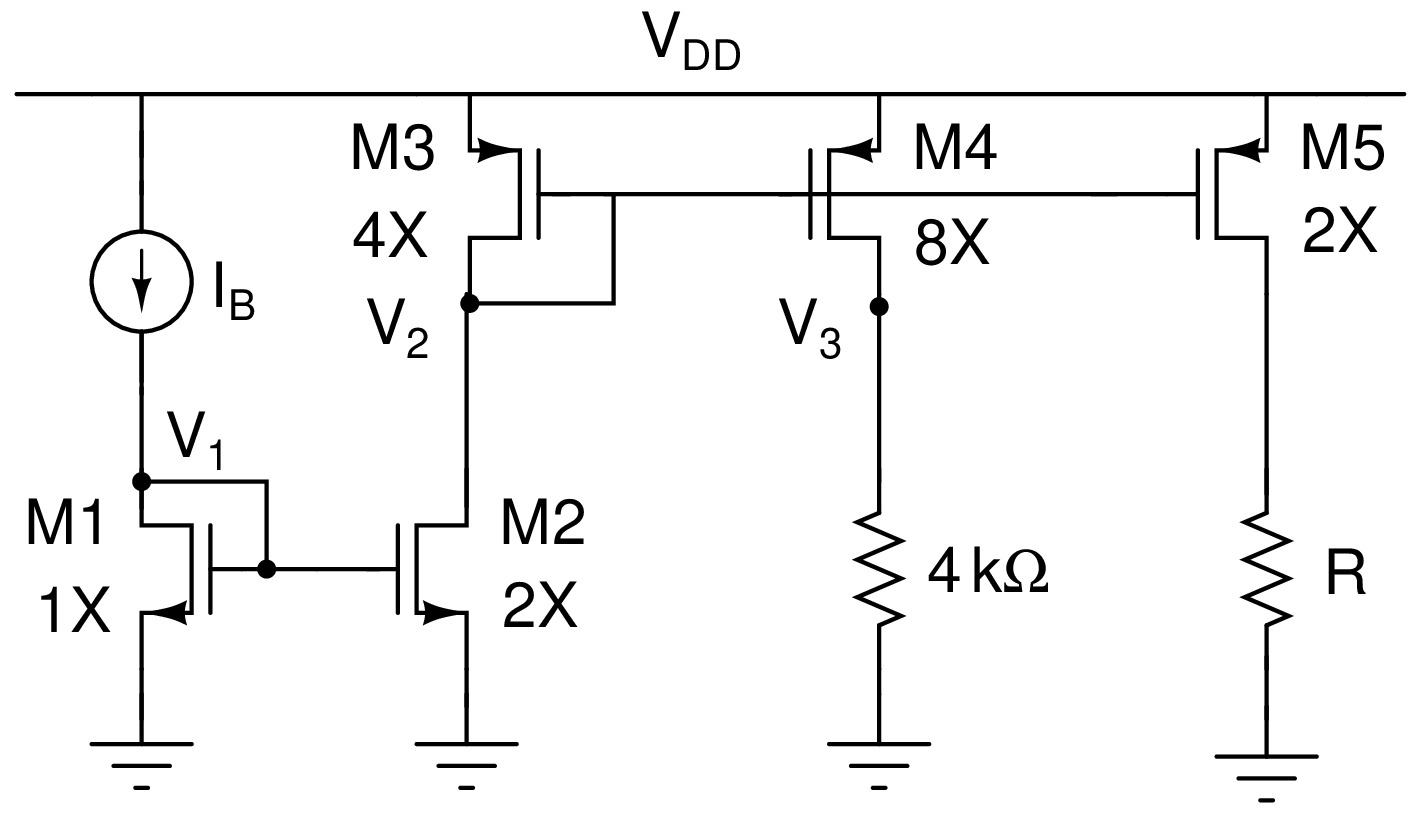
\includegraphics[width=0.7\textwidth]{figures/cc_dc_2 (1).jpg}
\end{center}
\end{figure}
\begin{enumerate}[label=\textbf{(\alph*)}]
    \item Determine the DC voltages $V_1$, $V_2$, and $V_3$.
$$V_{\rm OV1} = \sqrt{\frac{2I_{B}}{\mu_nC_{ox}(100/1)}} = 0.2\text{ V}$$
$$V_1 = V_{OV1} + V_{TN}$$
$$\boxed{V_1 = 1.2\text{ V}}$$
$$I_{D2} = 2I_B = 2(200)\ \mu\text{A}$$
$$V_{OV3} = 0.2 \text{ V}$$
$$V_2 = V_{DD} - V_{OV3} - |V_{TP}|$$
$$\boxed{V_2 = 3.8\text{ V}}$$
$$I_{D4} = 4I_B = 800\ \mu \rm A$$
$$V_{3} = I_{D4}(4\rm k)$$
$$\boxed{V_3 = 3.2\text{ V}}$$
\newpage
    \item Determine the value of R such that M5 is biased at the edge of saturation.
$$I_{D5} = I_B = 200\ \mu \rm A$$
$$V_{OV5} = 5 - I_{D5}R = 0.2\text{ V}$$
$$R = \frac{4.8}{200 \mu}$$
$$\boxed{R = 24 \text{ k} \Omega}$$
\end{enumerate}
\newpage
\subsection*{Problem 2}
For this problem, refer to the circuit below.
\begin{figure}[!htb]
\begin{center}
    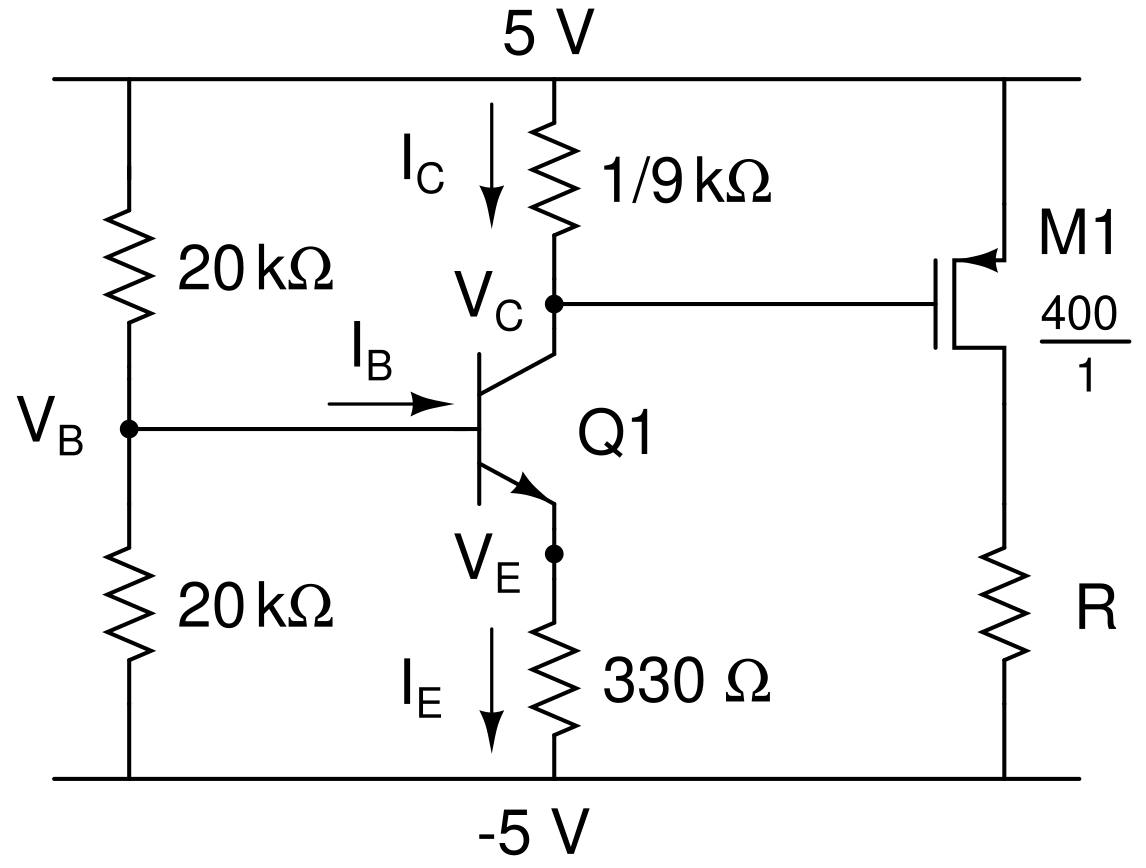
\includegraphics[width=0.6\textwidth]{figures/cc_dc1 (1).png}
\end{center}
\end{figure}
\begin{enumerate}[label=\textbf{(\alph*)}]
    \item Determine the DC currents and voltages $V_B$, $V_E$, $V_C$, $I_B$, $I_E$, and $I_C$ of Q1.  What is its region of operation?
    \\

\textbf{Solution:} \\
Convert the biasing network at the base of Q1 to its Thevenin equivalent:
$$V_{TH} = \left(5- (-5)\right)\left(\frac{20 \rm k}{20 \rm k + 20 k}\right) - 5 = 0\text{ V}$$
$$R_{TH} = 20\text{k} || 20\text{k} = 10\text{ k}\Omega$$
\newpage
The circuit can then be simplified to be:
\begin{figure}[!h]
\begin{center}
    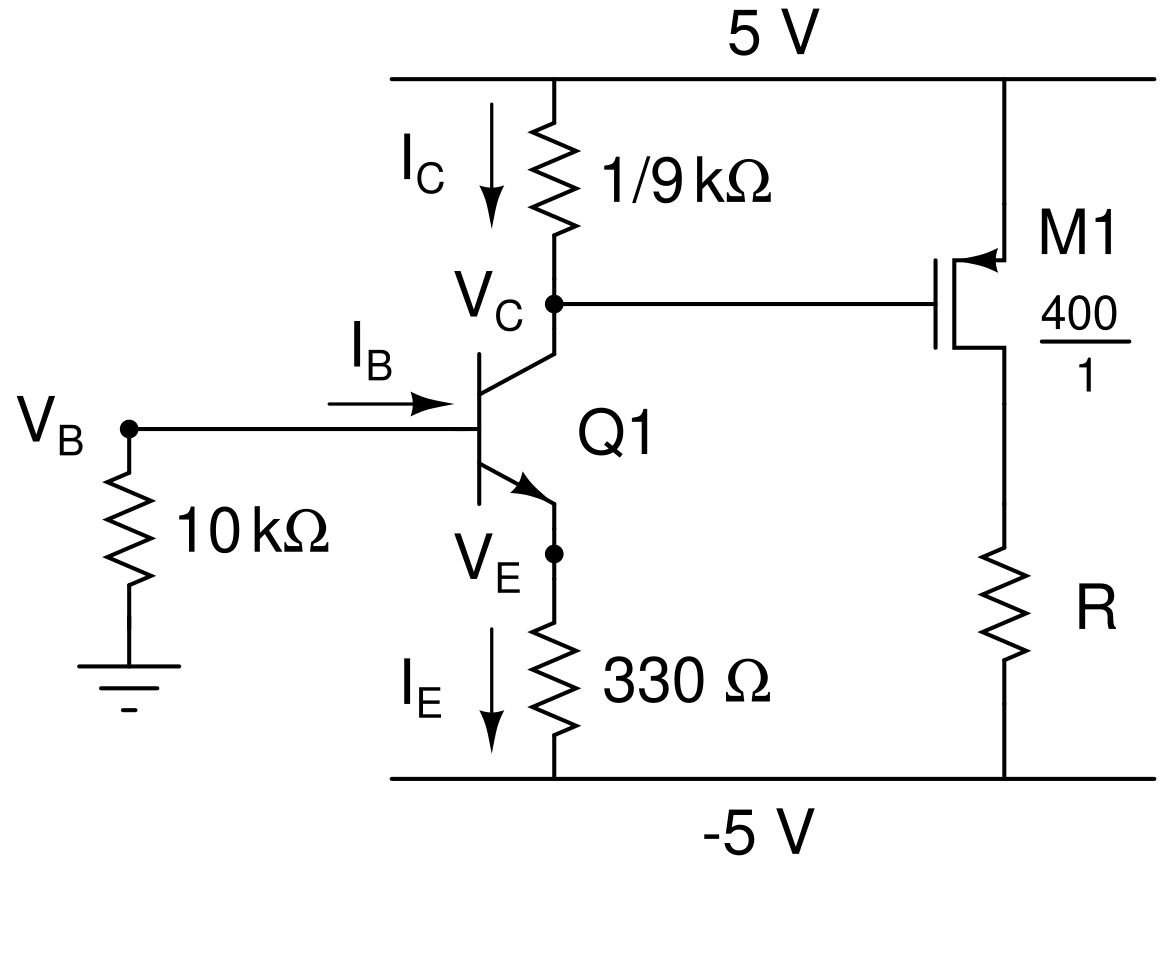
\includegraphics[width=0.6\textwidth]{figures/cc_dc1_sol.png}
\end{center}
\end{figure}
$$I_E = \frac{-I_B(10\text{k}) - 0.7 - (-5)}{330}$$
$$330(\beta + 1)I_B = -I_B(10\text{k}) - 0.7 - (-5)$$
$$I_B(33\text{k} + 10\text{k}) = 4.3$$
$$\boxed{I_B = 100\ \mu\text{A}}$$
$$\boxed{I_E = (\beta + 1)I_B = 10\text{ mA}}$$
$$\boxed{I_C = \beta I_B = 9.9\text{ mA}}$$
$$\boxed{V_{B} = -(10 \text{k})I_B = -1\text{ V}}$$
$$\boxed{V_{E} = -5 + (330)I_E = -1.7\text{ V}}$$
$$\boxed{V_{C} = 5 - (1/9)\text{k}I_C = 3.9\text{ V}}$$
$$V_{CE} = 5.6\text{ V} > V_{BE} = 0.7 \text{ V}$$
Q1 is operating in forward active mode.
    \item Determine the value of R such that M1 is biased at the edge of saturation.
$$V_{\rm OV1} = 5 - V_C - |V_{TP}| = 0.1$$
$$I_{D1} = \frac{\mu_p C_{ox}}{2}\left(\frac{400}{1}\right)V_{\rm OV1}^2 = \frac{5 - V_{OV1} - (-5)}{R}$$
$$100\mu R = 9.9$$
$$\boxed{R = 99\text{ k}\Omega}$$
\end{enumerate}
\newpage
\section*{Small-Signal Analysis}
\subsection*{Problem 1}
Determine the values of $G_M$, $R_{OUT}$, and $A_v = v_{out}/v_{in}$ of this amplifier.  Assume all MOSFETs are biased in saturation.  Do not assume $r_{ds} = \infty$, though you can assume $g_mr_{ds} >> 1$.
\begin{figure}[!h]
\begin{center}
    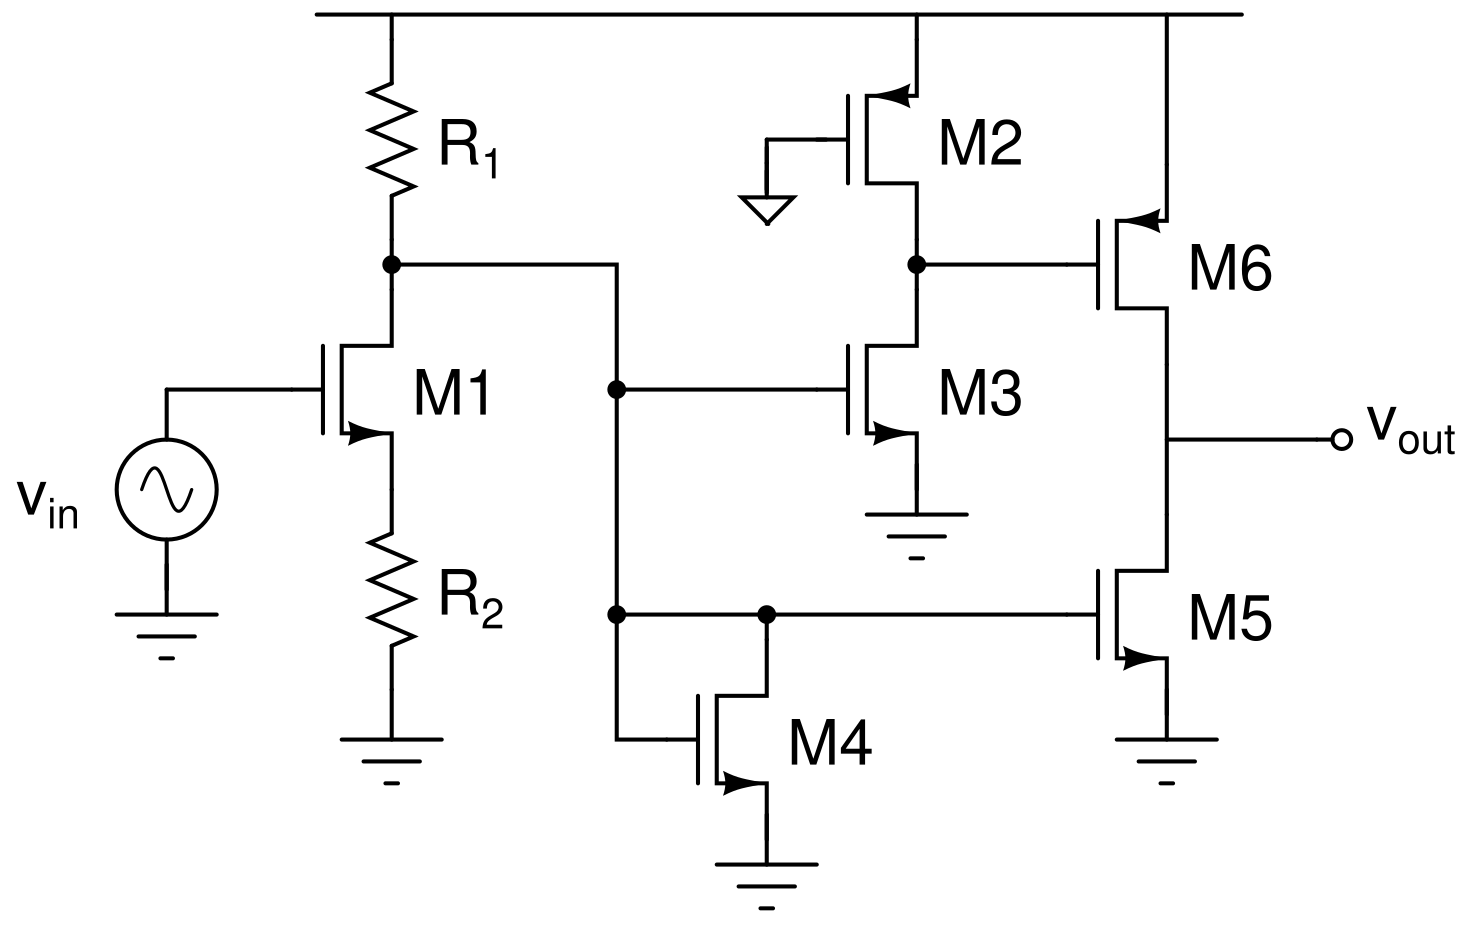
\includegraphics[width=0.85\textwidth]{figures/cc_amp1.png}
\end{center}
\end{figure} \\
\textbf{Solution: }
For such problems, it is often advantageous to break down the problem into multiple stages, find the gain of that particular part, and multiply with gain of subsequent state, etc. \\
Let $A_{v1}$ be defined as gain at the drain of M1. Then,   
$$G_{M1} = \frac{g_{m1}}{(1+g_{m1}R_2)}$$ 
$$R_{OUT1} = (1/g_{m4})  ||  (R_1) || (r_{ds1} + R_2 + g_{m1}r_{ds1}R_2)$$
$$A_{v1} = -G_{M1}R_{OUT1}$$
$$$$
Let $A_{v3}$ be defined as gain at the drain of M3: 
$$G_{M3} = g_{m3}$$
$$R_{OUT3} = r_{ds2}  ||  r_{ds3} $$
$$A_{v3} = -G_{M3}R_{OUT3}$$
Then by ${i_d = g_m  v_{gs}}$:
$$G_M = A_{v1}A_{v3}g_{m6} + A_{v1}g_{m5}$$
$$R_{OUT} = r_{ds5} || r_{ds6}$$
$$A_v = -G_{M}R_{OUT}$$
\newpage
\subsection*{Problem 2}
Determine the values of $G_M$, $R_{OUT}$, and $A_v = v_{out}/v_{in}$ of this amplifier.  Assume all MOSFETs are biased in saturation, all BJTs are biased in forward active mode, $r_{ds} \ne \infty$, $r_0 = \infty$, and $g_mr_{ds} \gg 1$.
\begin{figure}[!h]
\begin{center}
    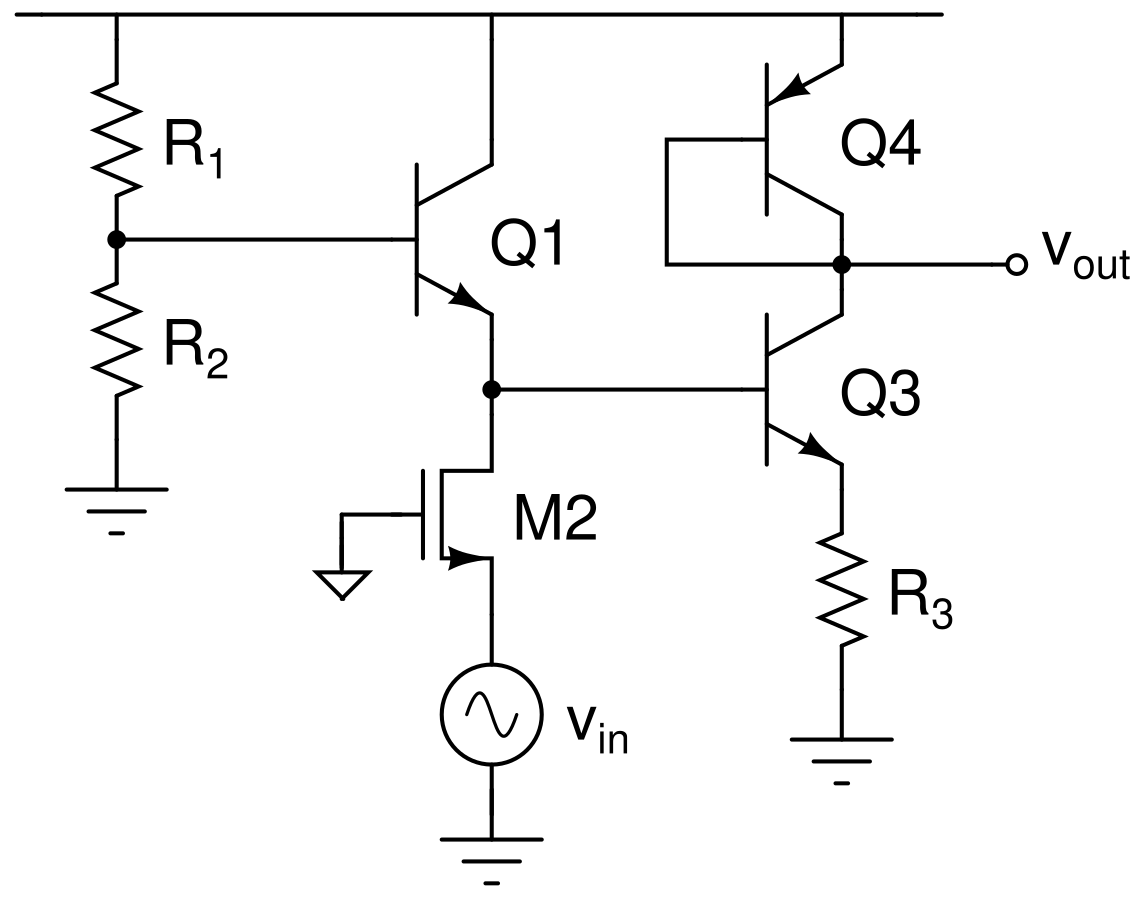
\includegraphics[width=0.65\textwidth]{figures/cc_amp_2.png}
\end{center}
\end{figure}\\
\textbf{Solution:}
$$G_{M1} = -g_{m2}$$
$$R_{\rm OUT1} = r_{ds2}||\left(\frac{R_1||R_2 + r_{\pi 1}}{\beta + 1}\right)$$
$$A_{v1} = -G_{M1}R_{\rm OUT1}$$
$$G_{M2} = \frac{1}{\frac{\rm R_{OUT1} + r_{\pi 3}}{\beta} + \frac{\beta + 1}{\beta} R_3}$$
$$R_{\rm OUT2} = \frac{r_{\pi 4}}{\beta + 1}$$
$$A_{v2} = -G_{M2}R_{\rm OUT2}$$
$$A_{v} = A_{v1}A_{v2}$$
\newpage
\subsection*{Problem 3}
Determine the values of $G_M$, $R_{OUT}$, and $A_v = v_{out}/v_{in}$ of this amplifier.  Assume all MOSFETs are biased in saturation, all BJTs are biased in forward active mode, $r_{ds} \ne \infty$, $r_0 = \infty$, and $g_mr_{ds} \gg 1$.
\begin{figure}[!h]
\begin{center}
    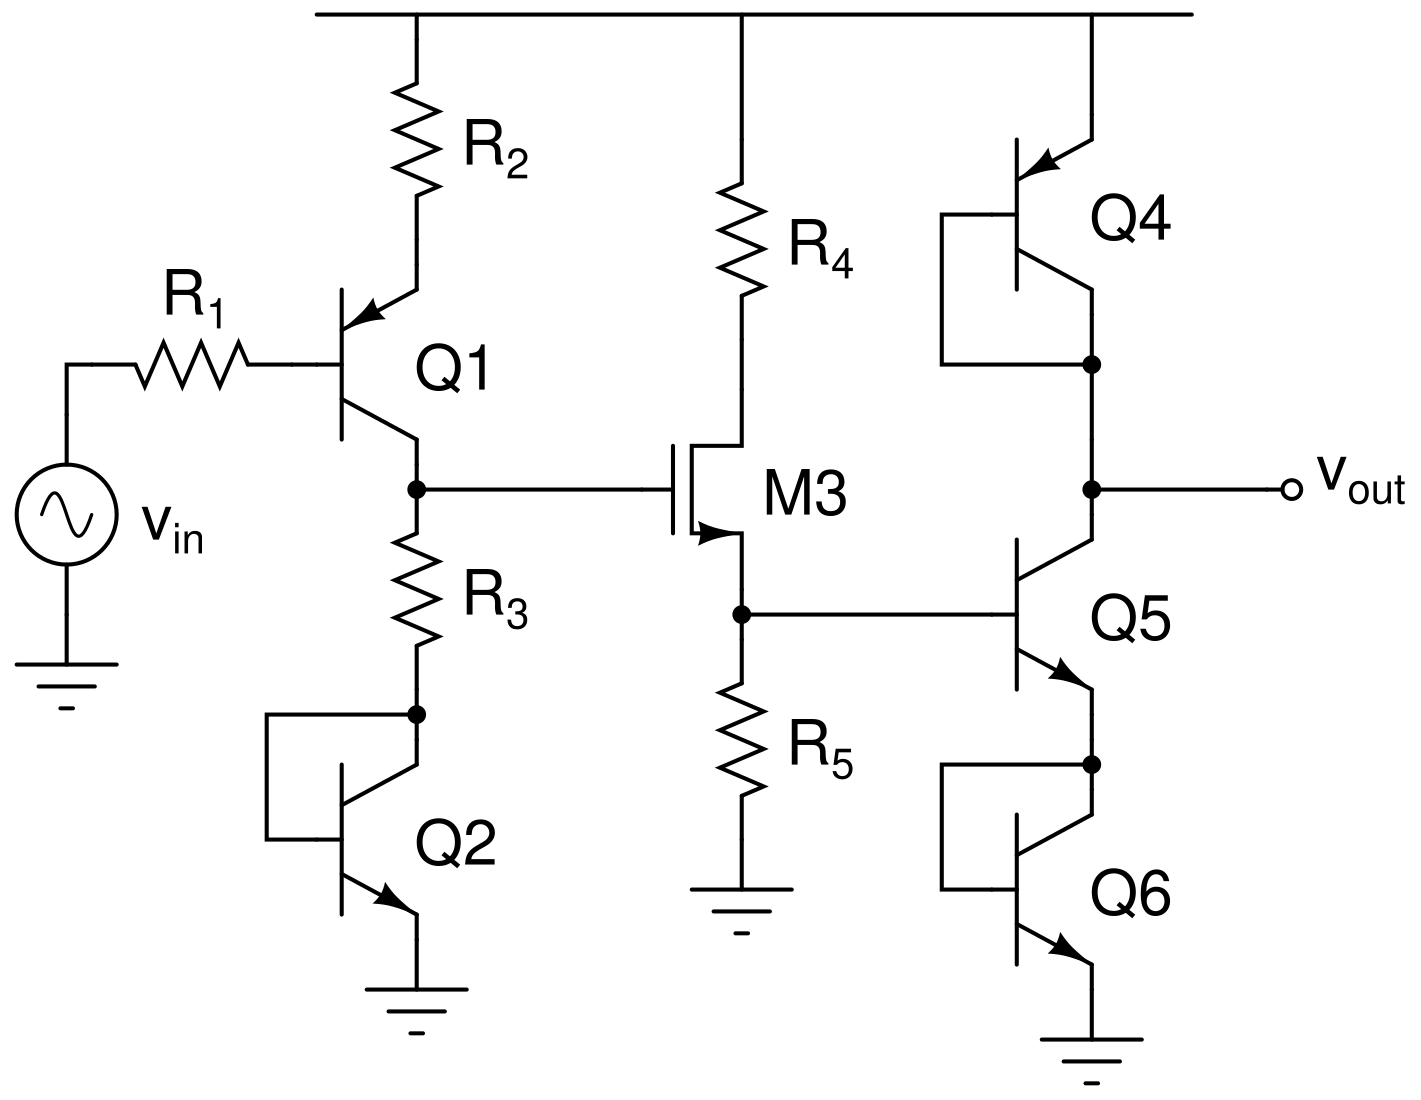
\includegraphics[width=0.75\textwidth]{figures/cc_amp_3.png}
\end{center}
\end{figure} \\
\textbf{Solution:}
At the gate of M3,
$$G_{M1} = \frac{1}{\frac{\rm R_{1} + r_{\pi 1}}{\beta_1} + \frac{\beta_1 + 1}{\beta_1} R_2} $$
$$R_{\rm OUT1} = \frac{r_{\pi 2}}{\beta_2 + 1} + R_3$$
$$A_{v1} = -G_{M1}R_{\rm OUT1}$$
At the source of M3,
$$G_{M2} = -\frac{g_{m3}}{1+\frac{R_4}{r_{ds3}}}$$
$$R_{\rm OUT2} = \frac{1}{g_{m3}} (1 + \frac{R_4}{r_{ds3}}) || R_5$$
$$A_{v2} = -G_{M2}R_{\rm OUT2}$$
The last branch is basically repeat of first branch.
$$G_{M3} = \frac{1}{\frac{\rm  r_{\pi 5} + R_{OUT2}}{\beta_5} + \frac{\beta_5 + 1}{\beta_5} R_y}$$
$$R_y = \frac{r_{\pi 6}}{\beta_6 + 1}$$
$$A_{v3} = -G_{m3}R_{\rm out3}$$
$$A_{v} = A_{v1}A_{v2}A_{v3}$$
\newpage
\subsection*{Problem 4}
Determine the values of $G_M$, $R_{OUT}$, and $A_v = v_{out}/v_{in}$ of this amplifier.  Assume all MOSFETs are biased in saturation.  Do not assume $r_{ds} = \infty$, though you can assume $g_mr_{ds} >> 1$.
\begin{figure}[!h]
\begin{center}
    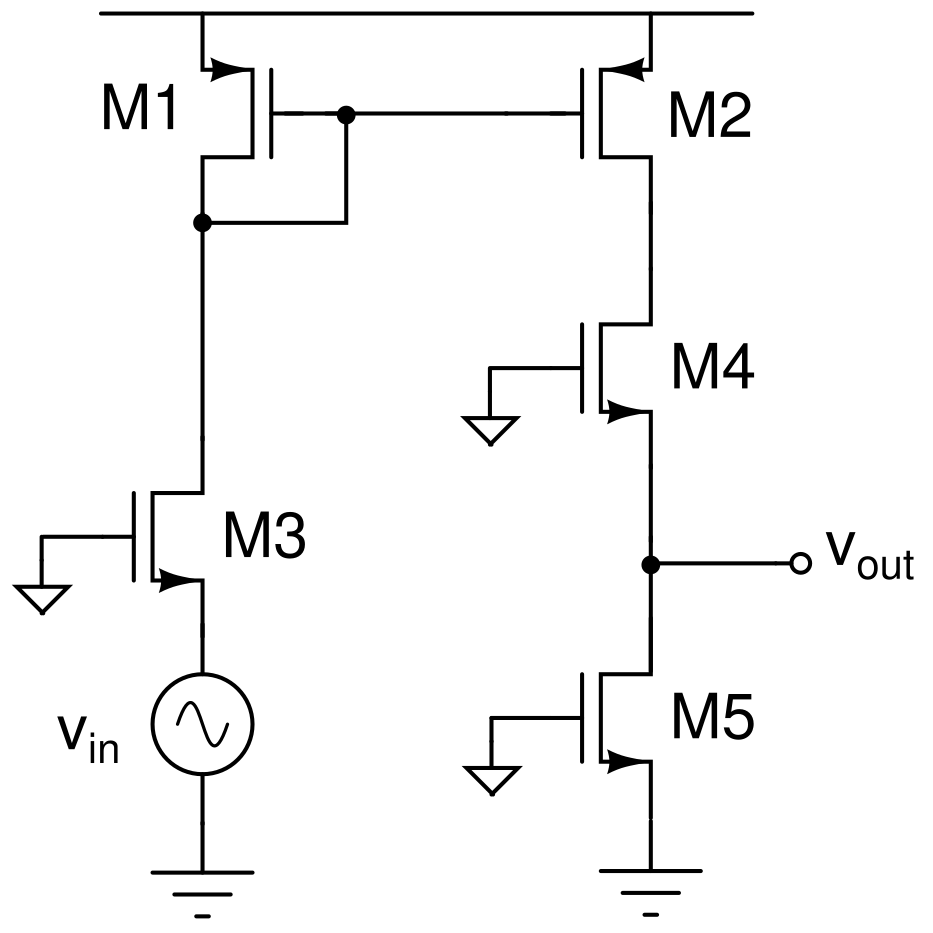
\includegraphics[width=0.5\textwidth]{figures/cc_amp_4.png}
\end{center}
\end{figure}
$$G_{M1} = -g_{m3}$$
$$R_{OUT1} = r_{ds3} || \left(\frac{1}{g_{m1}}\right)$$
$${A_{v1} = -G_{M1}R_{OUT1}}$$
$$\boxed{G_{M} = A_{v1}g_{m2}}$$
$$\boxed{R_{\rm OUT} = r_{ds5} || \left(\frac{1}{g_{m4}}\left(1 + \frac{r_{ds2}}{r_{ds4}}\right)\right)}$$
$$\boxed{A_{v} = -G_{M}R_{OUT}}$$
\newpage
\subsection*{Problem 5}
Determine the values of $G_M$, $R_{OUT}$, and $A_v = v_{out}/v_{in}$ of this amplifier.  Assume all MOSFETs are biased in saturation, all BJTs are biased in forward active mode, $r_{ds} \ne \infty$, $r_0 = \infty$, and $g_mr_{ds} \gg 1$. 
\begin{figure}[!h]
\begin{center}
    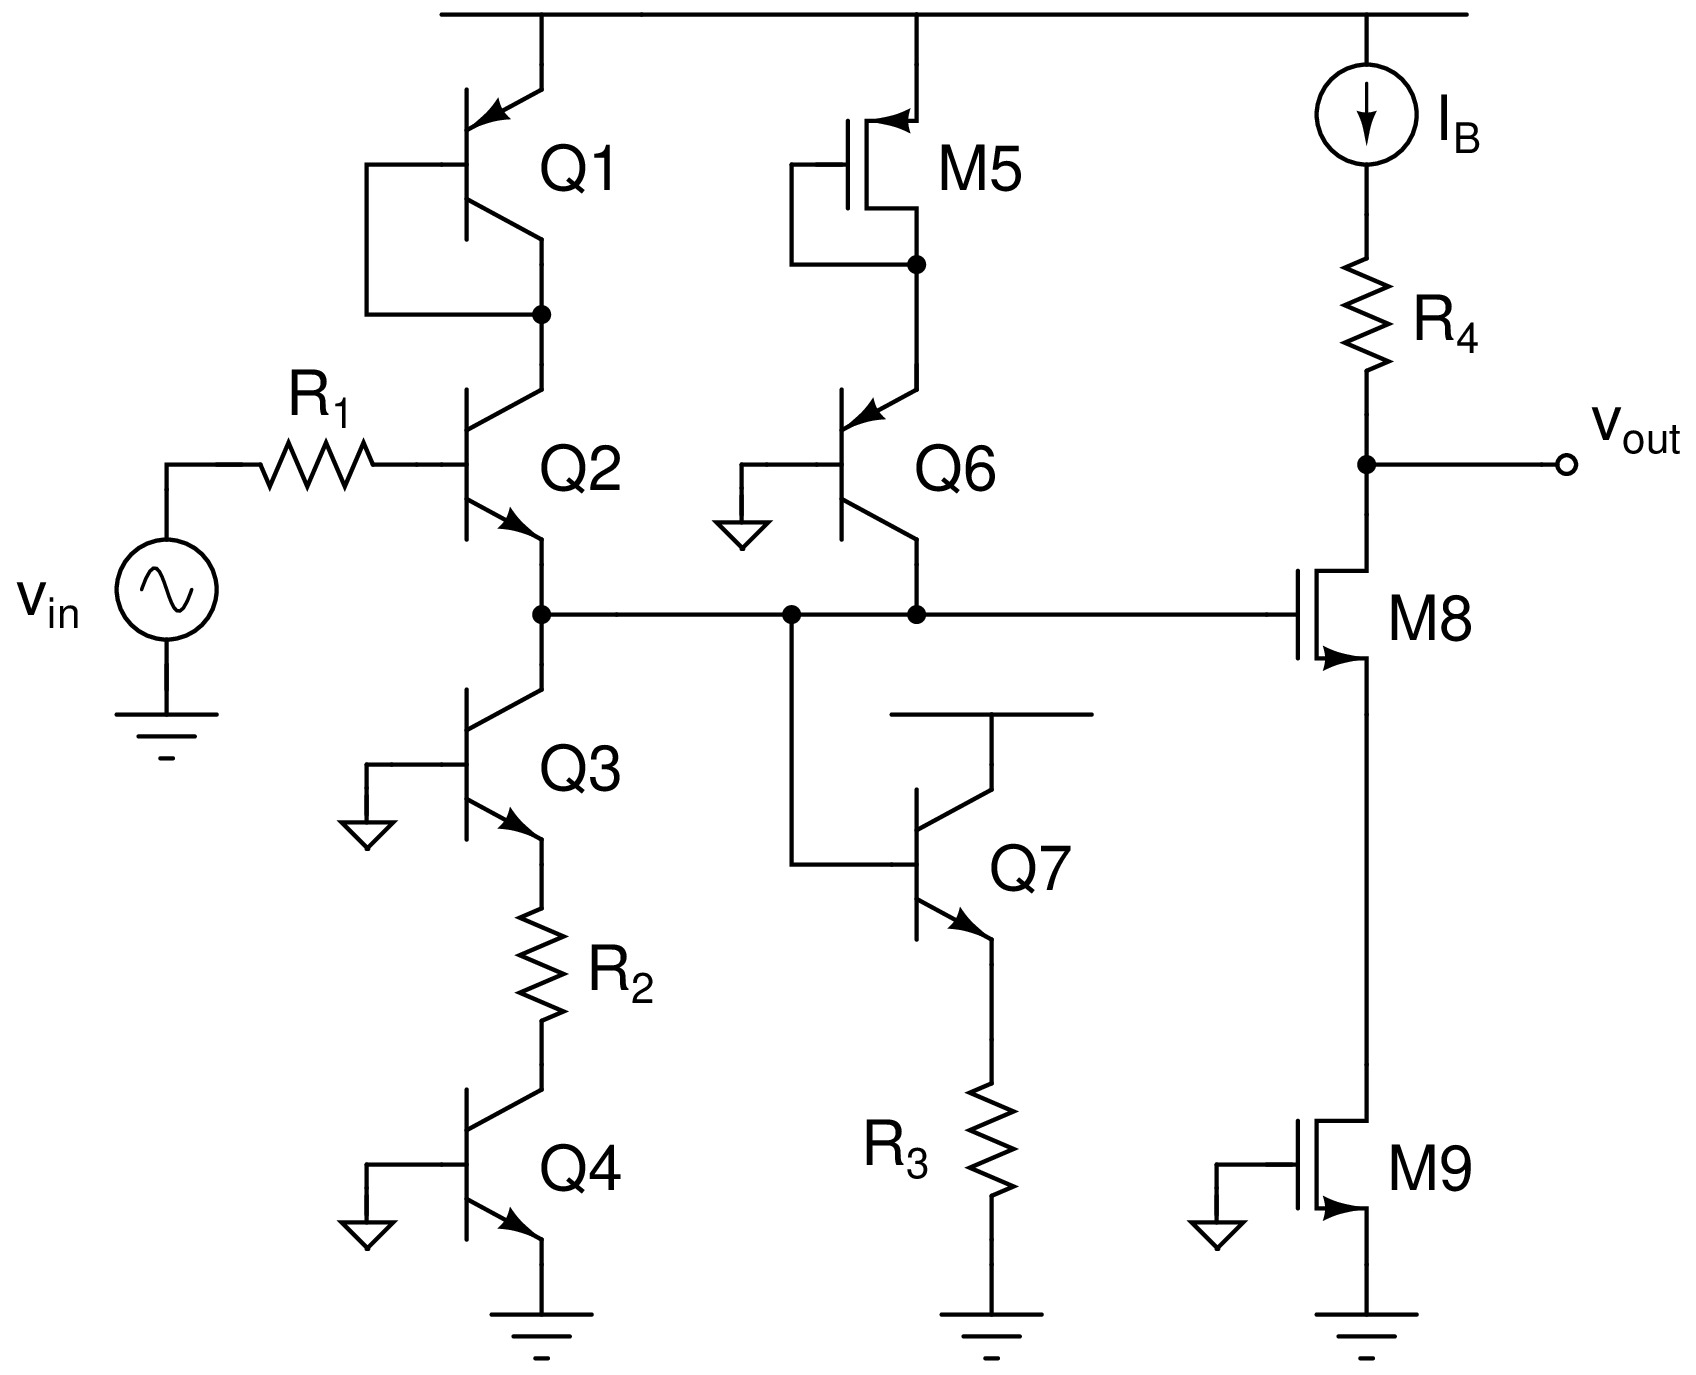
\includegraphics[width=0.8\textwidth]{figures/cc_amp5.jpg}
\end{center}
\end{figure}
$$G_{M1} = -\frac{1}{\frac{R_1 + r_{\pi2}}{\beta + 1} }$$
$$R_{OUT1}=\left(\frac{R_1 + r_{\pi2}}{\beta + 1}\right)||\left[r_{\pi 7} + (\beta + 1)R_3\right]$$
$$A_{v1} = -G_{M1}R_{OUT1}$$
$$\boxed{G_{M} = A_{v1}\frac{g_{m8}}{1 + g_{m8}r_{ds9}}}$$
$$\boxed{R_{OUT} = r_{ds8} + (1+g_{m8}r_{ds8})r_{ds9}}$$
$$\boxed{A_{v} = G_{M}R_{OUT}}$$

\newpage
\section*{Bode Plots}
\subsection*{Problem 1}
For the following amplifier transfer functions, \textbf{(i)} plot the magnitude response, \textbf{(ii)} determine the unity gain frequency, and \textbf{(iii)} plot the phase response:
\begin{enumerate}[label=\textbf{(\alph*)}]
    \item $$H(s) = \frac{10^4}{s(1+s/10^3)}$$
    \\ \textbf{Solution:}\\ \\
    \textbf{(i)} The magnitude response is plotted below:
    \begin{figure}[!h]
    \centering
    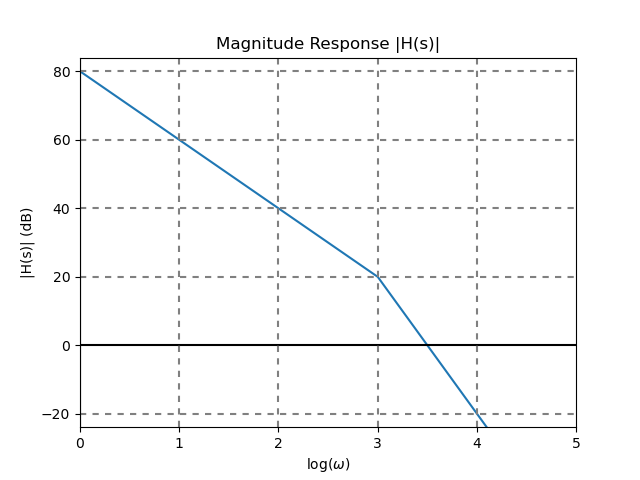
\includegraphics[width=0.7\textwidth]{figures/ece342_cc_mag_a.png}
    \end{figure} \\
    \textbf{(ii)} 
    $$\boxed{\omega_{ugf} = \sqrt{10} \cdot 10^3 \text{ rad/s}}$$
    \newpage
    \textbf{(iii)} The phase response is plotted below:
    \begin{figure}[!h]
    \centering
    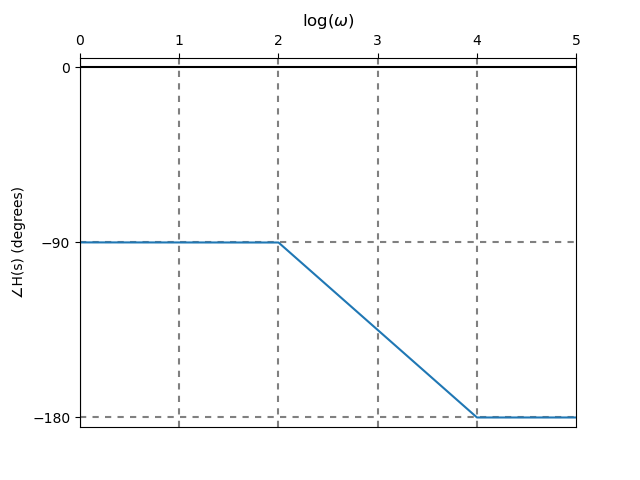
\includegraphics[width=0.7\textwidth]{figures/cc_phase_a.png}
    \end{figure}
    \item $$H(s) = \frac{2000\left(1 + \frac{s}{10^2}\right)}{\left(1 + \frac{s}{10}\right)\left(1 + \frac{s}{10^3}\right)\left(1 + \frac{s}{10^4}\right)}$$
    \\ \textbf{Solution:}\\ \\
    \textbf{(i)} The magnitude response is plotted below:
    \begin{figure}[!h]
    \centering
    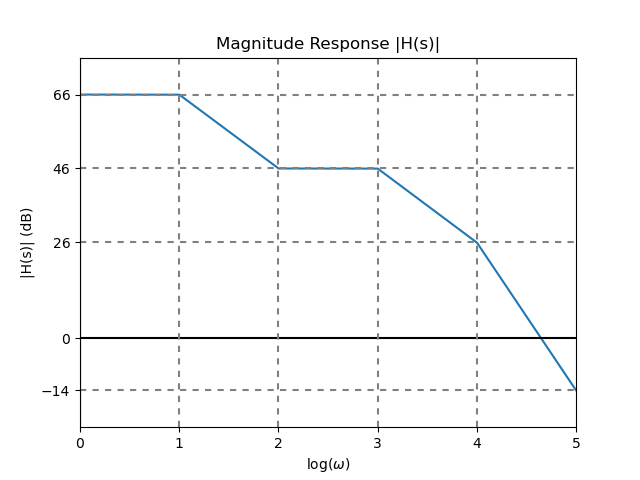
\includegraphics[width=0.7\textwidth]{figures/ece342_cc_mag.png}
    \end{figure} \newpage
    \textbf{(ii)} After $\omega = 10^4$ rad/s, the magnitude response decreases at 40 dB / decade, or 12 dB / octave.  Thus, $|H(s)|_{dB}$ =  6 dB at $\omega = \sqrt{10} \cdot 10^4$ rad/s.  Since the magnitude response decreases at 12 dB / octave, $|H(s)|_{dB}$ will be 0 dB at $\omega = \sqrt{2} \cdot \sqrt{10} \cdot 10^4$ rad/s.
    $$\boxed{\omega_{ugf} = \sqrt{20} \cdot 10^4 \text{ rad/s}}$$
    \textbf{(iii)} The phase response is plotted below:
    \begin{figure}[!h]
    \centering
    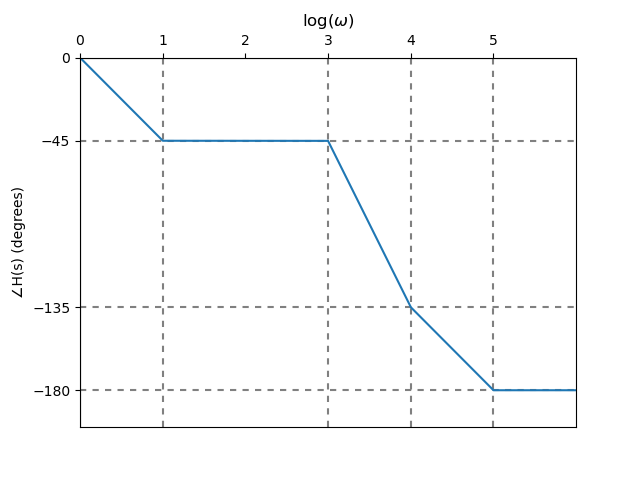
\includegraphics[width=0.7\textwidth]{figures/ece342_cc_phaseresponse.png}
    \end{figure}
    \newpage
    \item $$H(s) = \frac{4000(1+s/10^2)}{(1+s/10)(1+s/10^4)^2}$$
    \\ \textbf{Solution:}\\ \\
    \textbf{(i)} The magnitude response is plotted below:
    \begin{figure}[!h]
    \centering
    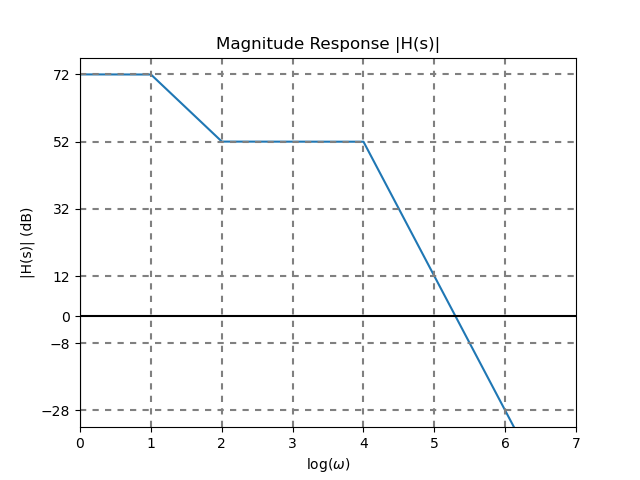
\includegraphics[width=0.7\textwidth]{figures/ece342_cc_mag_c.png}
    \end{figure} \\
    \textbf{(ii)} 
    $$\boxed{\omega_{ugf} = 2 \cdot 10^5 \text{ rad/s}}$$
    \newpage
    \textbf{(iii)} The phase response is plotted below:
    \begin{figure}[!h]
    \centering
    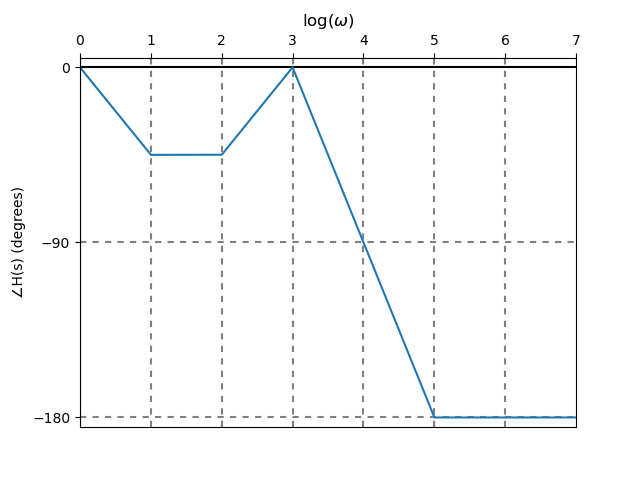
\includegraphics[width=0.7\textwidth]{figures/cc_phase_c.png}
    \end{figure}
\end{enumerate}
\newpage
\subsection*{Problem 2}
For each of the amplifier transfer functions in Problem 1, determine the incremental output voltage response $v_{out}(t)$ to an incremental input voltage $v_{in}(t) = 10\cos(10^3 \cdot t)$ mV. \\ \\
\textbf{Solution:} \\
\begin{enumerate}[label=\textbf{(\alph*)}]
\item $$H(s) = \frac{10^4}{s(1+s/10^3)}$$
From the Bode plot:
$$|H(j10^3)| = 20\text{ dB} = 10\text{ V/V}$$
$$\angle H(j10^3) = -135^{\circ}$$
$$v_{out}(t) = 10\cdot |H(j10^3)| \cos(10^3 \cdot t + \angle H(j10^3))\text{ mV}$$
$$\boxed{v_{out}(t) = 100 \cos(10^3 \cdot t -135^{\circ})\text{ mV}}$$
\item $$H(s) = \frac{2000\left(1 + \frac{s}{10^2}\right)}{\left(1 + \frac{s}{10}\right)\left(1 + \frac{s}{10^3}\right)\left(1 + \frac{s}{10^4}\right)}$$
From the Bode plot: 
$$|H(j10^3)| = 46\text{ dB} = 200\text{ V/V}$$
$$\angle H(j10^3) = -45^{\circ}$$
$$v_{out}(t) = 10\cdot |H(j10^3)| \cos(10^3 \cdot t + \angle H(j10^3))\text{ mV}$$
$$\boxed{v_{out}(t) = 2 \cos(10^3 \cdot t -45^{\circ})\text{ V}}$$
\item $$H(s) = \frac{4000(1+s/10^2)}{(1+s/10)(1+s/10^4)^2}$$
From the Bode plot: 
$$|H(j10^3)| = 52\text{ dB} = 400\text{ V/V}$$
$$\angle H(j10^3) = 0^{\circ}$$
$$v_{out}(t) = 10\cdot |H(j10^3)| \cos(10^3 \cdot t + \angle H(j10^3))\text{ mV}$$
$$\boxed{v_{out}(t) = 4 \cos(10^3 \cdot t)\text{ V}}$$
\end{enumerate}
\newpage
\section*{Open Circuit Time Constants}
\subsection*{Problem 1}
Use the open-circuit time constant method to estimate the -3 dB frequency, $\omega_{\rm -3 dB}$, of this amplifier.  Consider $C_{gs}$, $C_{gd}$, $C_{\pi}$, $C_{\mu}$, and $r_{ds}$.  Ignore $r_0$. \\ 
\begin{figure}[!h]
\begin{center}
    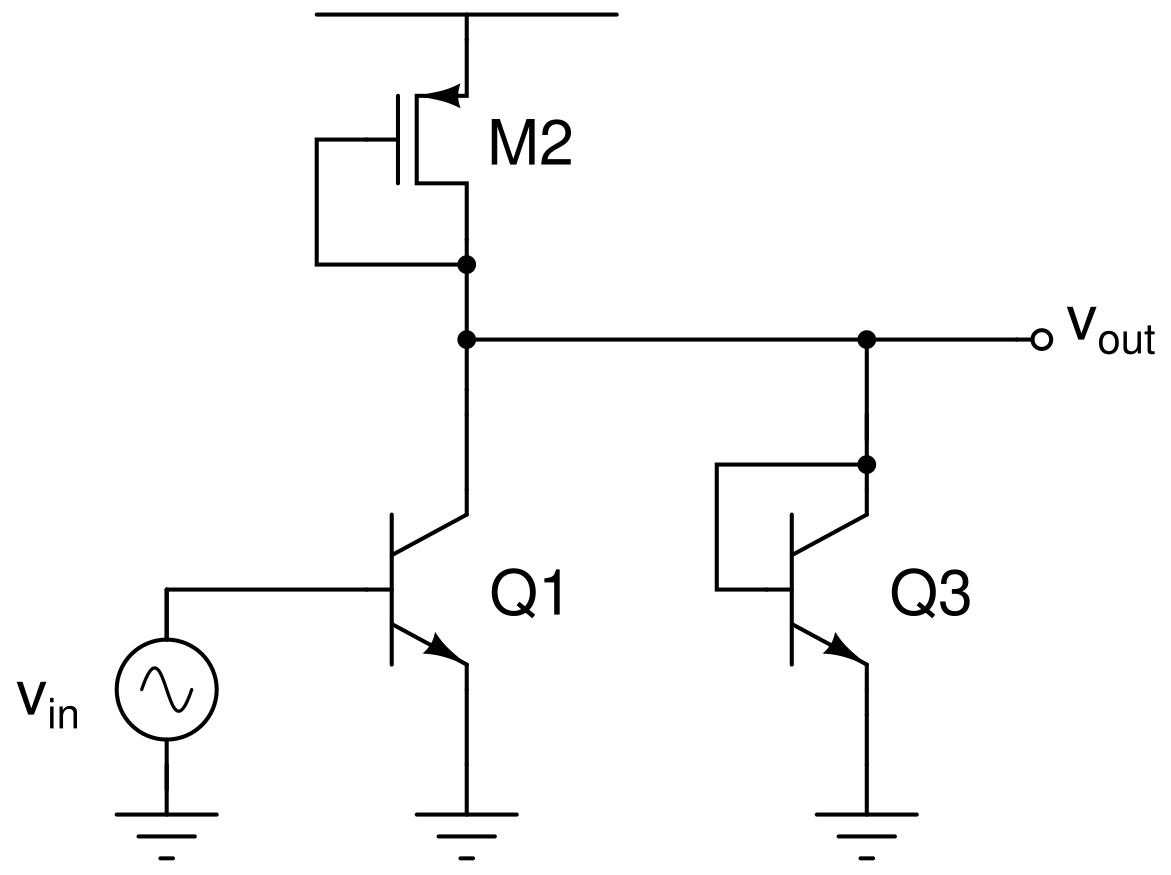
\includegraphics[width=0.65\textwidth]{figures/cc_octc2.png}
\end{center}
\end{figure} \\
\textbf{Solution:} \\
$\tau_{C_{\pi 1}}$:
$$R_{C_{\pi 1}} = 0$$
$$\boxed{\tau_{C_{\pi 1}} = 0}$$
$\tau_{C_{\mu 1}}$:
$$R_{C_{\mu 1}} = \left(\frac{1}{g_{m2}}\right) || \left(\frac{r_{\pi 3}}{\beta + 1}\right) $$
$$\boxed{\tau_{C_{\mu 1}} = \left[\left(\frac{1}{g_{m2}}\right) || \left(\frac{r_{\pi 3}}{\beta + 1}\right)\right]C_{\mu 1}}$$
$\tau_{C_{gs2}}$:
$$R_{C_{gs2}} = \left(\frac{1}{g_{m2}}\right) || \left(\frac{r_{\pi 3}}{\beta + 1}\right) $$
$$\boxed{\tau_{C_{gs2}} = \left[\left(\frac{1}{g_{m2}}\right) || \left(\frac{r_{\pi 3}}{\beta + 1}\right)\right]C_{gs 2}}$$
$\tau_{C_{gd2}}$:
$$R_{C_{gd2}} = 0$$
$$\boxed{\tau_{C_{gd2}} = 0}$$
$\tau_{C_{\pi 3}}$:
$$R_{C_{\pi 3}} = \left(\frac{1}{g_{m2}}\right) || \left(\frac{r_{\pi 3}}{\beta + 1}\right) $$
$$\boxed{\tau_{C_{\pi 3}} = \left[\left(\frac{1}{g_{m2}}\right) || \left(\frac{r_{\pi 3}}{\beta + 1}\right)\right]C_{\pi 3}}$$
$\tau_{C_{\mu 3}}$:
$$R_{C_{\mu 3}} = 0 $$
$$\boxed{\tau_{C_{\mu 3}} = 0}$$
$$\omega_{\rm -3dB} = \frac{1}{\tau_{C_{\pi 1}} + \tau_{C_{\mu 1}} + \tau_{C_{gs2}} + \tau_{C_{gd2}} + \tau_{C_{\pi 3}} + \tau_{C_{\mu 3}}}$$
$$\boxed{\omega_{\rm -3 dB} = \frac{1}{\left[\left(\frac{1}{g_{m2}}\right) || \left(\frac{r_{\pi 3}}{\beta + 1}\right)\right](C_{\mu 1} + C_{gs 2} + C_{\pi 3})}}$$
\newpage
\subsection*{Problem 2}
Use the open-circuit time constant method to estimate the -3 dB frequency, $\omega_{\rm -3 dB}$, of this amplifier.  Consider $C_{gs}$, $C_{gd}$, $C_{\pi}$, $C_{\mu}$, and $r_{ds}$.  Ignore $r_0$. \\ 
\begin{figure}[!h]
\begin{center}
    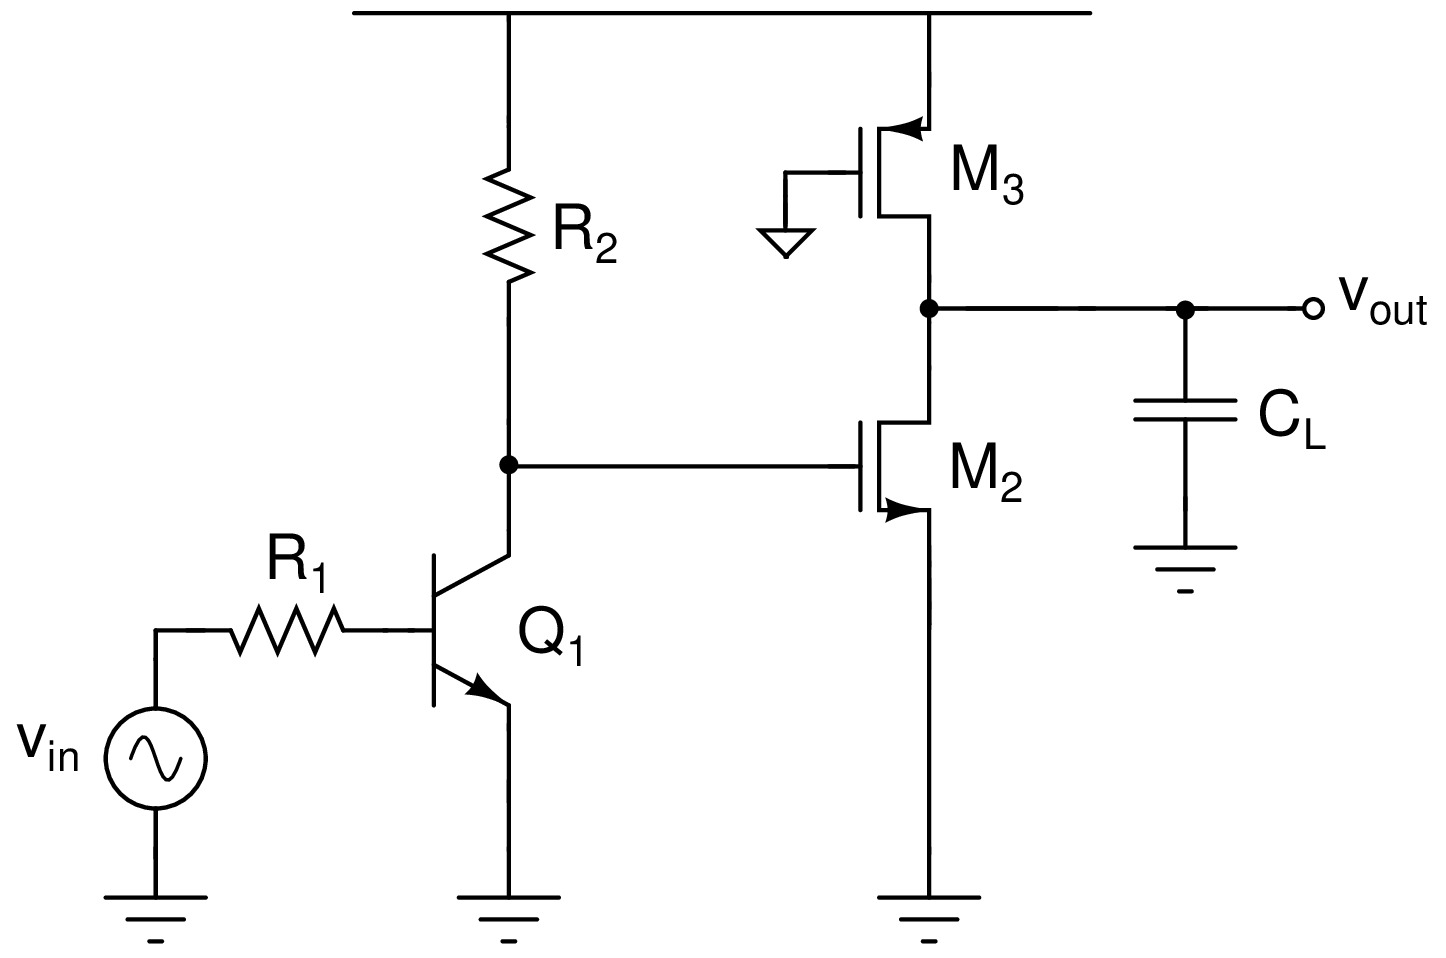
\includegraphics[width=0.7\textwidth]{figures/cc_octc1.jpg}
\end{center}
\end{figure} \\
\textbf{Solution:} \\
$\tau_{C_{\pi}}$:
$$R_{C_{\pi}} = R_1 || r_{\pi 1}$$
$$\boxed{\tau_{C_{\pi}} = \left(R_1 || r_{\pi 1}\right)C_{\pi}}$$
$\tau_{C_{\mu}}$:
$$R_{left} = R_1 || r_{\pi 1}$$
$$R_{right} = R_2$$
$$G_M = \frac{1}{\frac{r_{\pi 1}}{\beta _1}} = g_{m1}$$
$$R_{C_{\mu}} = R_{left} + R_{right} + G_MR_{left}R_{right}$$
$$\boxed{R_{C_{\mu}} = R_1 || r_{\pi 1} + R_2 + g_{m1}\left(R_1 || r_{\pi 1}\right)R_2}$$
$$\boxed{\tau_{C_{\mu}} = R_{C_{\mu}}C_{\mu}}$$
$\tau_{C_{gs2}}$:
$$R_{C_{gs2}} = R_2$$
$$\boxed{\tau_{C_{gs2}} = R_2C_{gs2}}$$
$\tau_{C_{gd2}}$:
$$R_{left} = R_2$$
$$R_{right} = r_{ds2}||r_{ds3}$$
$$G_M = g_{m2}$$
$$R_{C_{gd2}} = R_2 + R_{right} + G_MR_{left}R_{right}$$
$$\boxed{R_{C_{gd2}} = R_2 + r_{ds2}||r_{ds3} + g_{m2}R_2\left(r_{ds2}||r_{ds3}\right)}$$
$$\boxed{\tau_{C_{gd2}} = R_{C_{gd2}}C_{gd2}}$$
$\tau_{C_{gs3}}$:
$$R_{C_{gs3}} = 0$$
$$\boxed{\tau_{C_{gs3}} = 0}$$
$\tau_{C_{gd3}}$:
$$R_{C_{gd3}} = r_{ds2}||r_{ds3}$$
$$\boxed{\tau_{C_{gd3}} = \left(r_{ds2}||r_{ds3}\right)C_{gd3}}$$

$\tau_{C_L}$:
$$R_{C_L} = r_{ds2}||r_{ds3}$$
$$\boxed{\tau_{C_L} = \left(r_{ds2}||r_{ds3}\right)C_{L}}$$

Using the OCTC method:
$$\boxed{\omega_{\rm -3dB} = \frac{1}{\tau_{C_{\pi}} + \tau_{C_{\mu}} + \tau_{C_{gs2}} + \tau_{C_{gd2}} + \tau_{C_{gs3}} + \tau_{C_{gd3}} + \tau_{C_L}}}$$
\newpage
\subsection*{Problem 3}
Use the open-circuit time constant method to estimate the -3 dB frequency, $\omega_{\rm -3 dB}$, of this amplifier.  Consider $C_{gs}$, $C_{gd}$, $C_{\pi}$, $C_{\mu}$, and $r_{ds}$. 
\begin{figure}[!h]
\begin{center}
    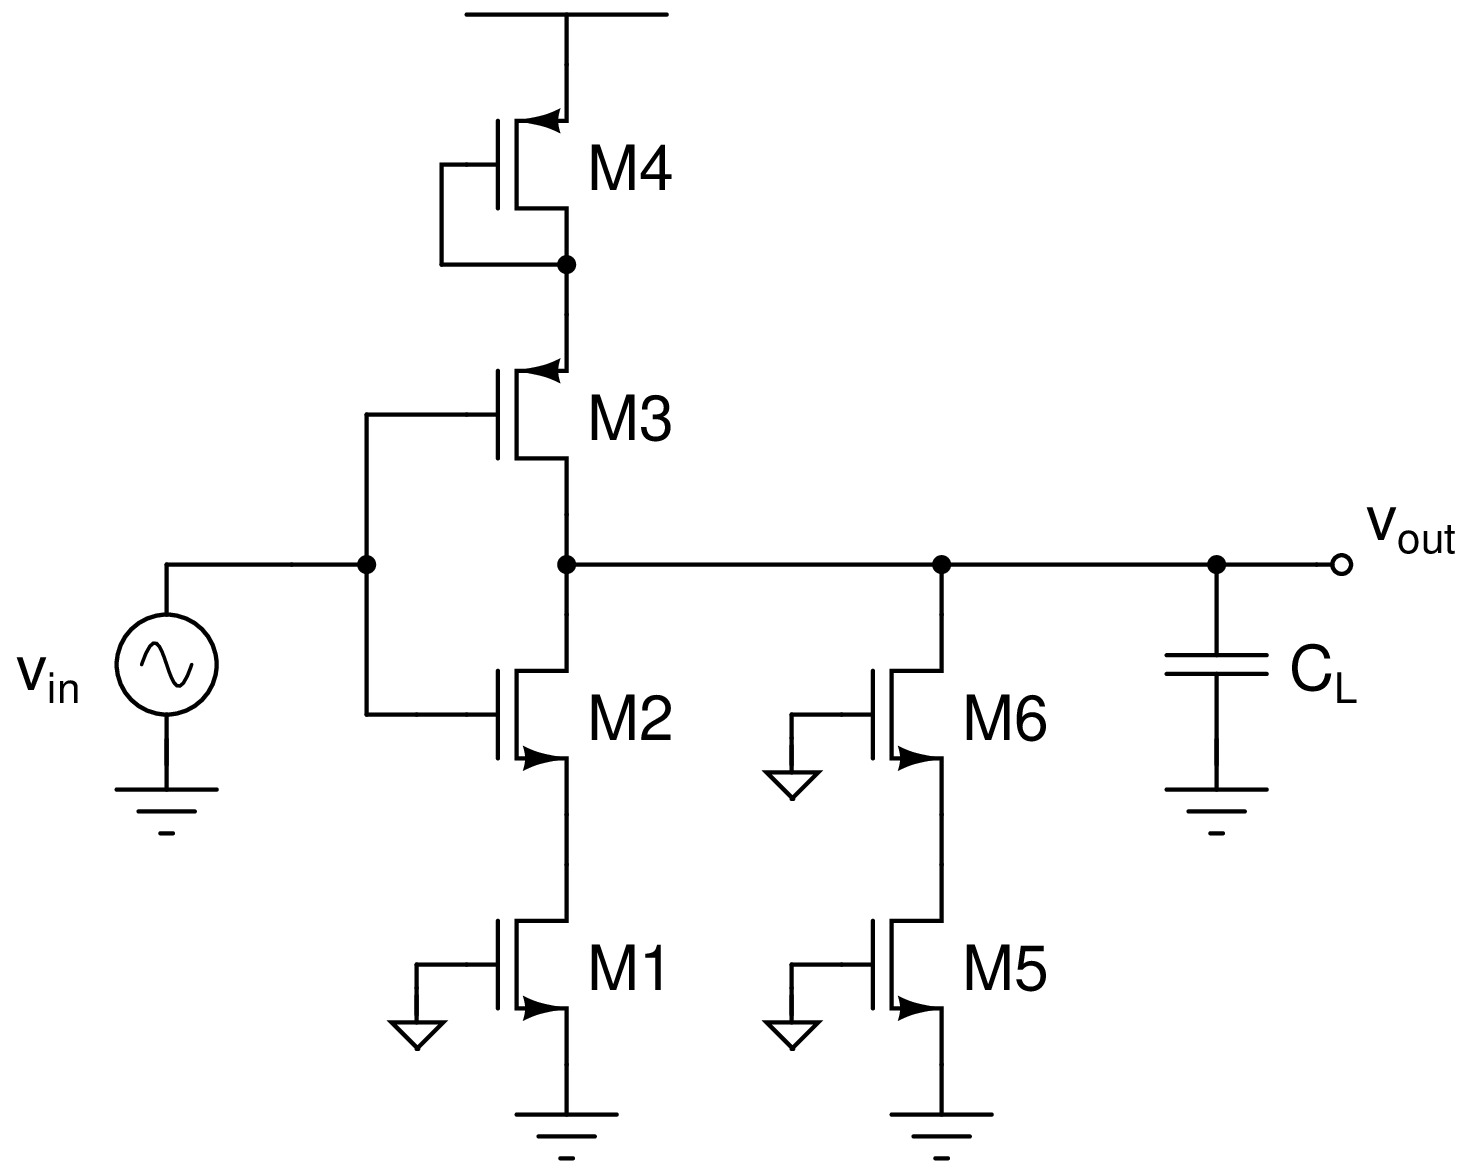
\includegraphics[width=0.7\textwidth]{figures/cc_octc3 (2).jpg}

\end{center}
\end{figure} \\
\textbf{Solution:} \\
$\tau_{C_{gs1}}$:
$$R_{C_{gs1}} = 0$$
$$\boxed{\tau_{C_{gs1}} = 0}$$
$\tau_{C_{gd1}}$:
$$R_{C_{gd1}} = \left[\frac{1}{g_{m2}}\left(1 + \frac{R_x}{r_{ds2}}\right)\right]||r_{ds1}$$
$$R_x = \left(r_{ds3} + \frac{1}{g_{m4}}\right) || \left[r_{ds6} + (1 + g_{m6}r_{ds6})r_{ds5}\right]$$
$$\boxed{\tau_{C_{gd1}} = R_{C_{gd1}}C_{gd1}}$$
$\tau_{C_{gs2}}$:
$$R_{C_{gs2}} = \left[\frac{1}{g_{m2}}\left(1 + \frac{R_x}{r_{ds2}}\right)\right]||r_{ds1}$$
$$R_x = \left(r_{ds3} + \frac{1}{g_{m4}}\right) || \left[r_{ds6} + (1 + g_{m6}r_{ds6})r_{ds5}\right]$$
$$\boxed{\tau_{C_{gs2}} = R_{C_{gs2}}C_{gs2}}$$
$\tau_{C_{gd2}}$:
$$R_{C_{gd2}} =  \left(r_{ds3} + \frac{1}{g_{m4}}\right) || \left[r_{ds2} + (1 + g_{m2}r_{ds2})r_{ds1}\right] || \left[r_{ds6} + (1 + g_{m6}r_{ds6})r_{ds5}\right]$$
$$\boxed{\tau_{C_{gd2}} = R_{C_{gd2}}C_{gd2}}$$
$\tau_{C_{gs3}}$:
$$R_{C_{gs3}} = \left[\frac{1}{g_{m3}}\left(1 + \frac{R_y}{r_{ds3}}\right)\right]||\left(\frac{1}{g_{m4}}\right)$$
$$R_y = \left[r_{ds2} + (1 + g_{m2}r_{ds2})r_{ds1}\right] || \left[r_{ds6} + (1 + g_{m6}r_{ds6})r_{ds5}\right]$$
$$\boxed{\tau_{C_{gs3}} = R_{C_{gs3}}C_{gs3}}$$
$\tau_{C_{gd3}}$:
$$R_{C_{gd3}} =  \left(r_{ds3} + \frac{1}{g_{m4}}\right) || \left[r_{ds2} + (1 + g_{m2}r_{ds2})r_{ds1}\right] || \left[r_{ds6} + (1 + g_{m6}r_{ds6})r_{ds5}\right]$$
$$\boxed{\tau_{C_{gd3}} = R_{C_{gd3}}C_{gd3}}$$
$\tau_{C_{gs4}}$:
$$R_{C_{gs4}} = \left[\frac{1}{g_{m3}}\left(1 + \frac{R_y}{r_{ds3}}\right)\right]||\left(\frac{1}{g_{m4}}\right)$$
$$R_y = \left[r_{ds2} + (1 + g_{m2}r_{ds2})r_{ds1}\right] || \left[r_{ds6} + (1 + g_{m6}r_{ds6})r_{ds5}\right]$$
$$\boxed{\tau_{C_{gs4}} = R_{C_{gs4}}C_{gs4}}$$
$\tau_{C_{gd4}}$:
$$R_{C_{gd4}} = 0$$
$$\boxed{\tau_{C_{gd4}} = 0}$$
$\tau_{C_{gs5}}$:
$$R_{C_{gs5}} = 0$$
$$\boxed{\tau_{C_{gs5}} = 0}$$
$\tau_{C_{gd5}}$:
$$R_{C_{gd5}} = \left[\frac{1}{g_{m6}}\left(1 + \frac{R_z}{r_{ds6}}\right)\right]||r_{ds5}$$
$$R_z = \left(r_{ds3} + \frac{1}{g_{m4}}\right) || \left[r_{ds2} + (1 + g_{m2}r_{ds2})r_{ds1}\right]$$
$$\boxed{\tau_{C_{gd5}} = R_{C_{gd5}}C_{gd5}}$$
$\tau_{C_{gs6}}$:
$$R_{C_{gs6}} = \left[\frac{1}{g_{m6}}\left(1 + \frac{R_z}{r_{ds6}}\right)\right]||r_{ds5}$$
$$R_z = \left(r_{ds3} + \frac{1}{g_{m4}}\right) || \left[r_{ds2} + (1 + g_{m2}r_{ds2})r_{ds1}\right]$$
$$\boxed{\tau_{C_{gs6}} = R_{C_{gs6}}C_{gs6}}$$
$\tau_{C_{gd6}}$:
$$R_{C_{gd6}} =  \left(r_{ds3} + \frac{1}{g_{m4}}\right) || \left[r_{ds2} + (1 + g_{m2}r_{ds2})r_{ds1}\right] || \left[r_{ds6} + (1 + g_{m6}r_{ds6})r_{ds5}\right]$$
$$\boxed{\tau_{C_{gd6}} = R_{C_{gd6}}C_{gd6}}$$
$\tau_{C_{L}}$:
$$R_{C_{L}} =  \left(r_{ds3} + \frac{1}{g_{m4}}\right) || \left[r_{ds2} + (1 + g_{m2}r_{ds2})r_{ds1}\right] || \left[r_{ds6} + (1 + g_{m6}r_{ds6})r_{ds5}\right]$$
$$\boxed{\tau_{C_{L}} = R_{C_{L}}C_{L}}$$

Using the OCTC method:
$$\boxed{\omega_{\rm -3dB} = \frac{1}{\tau_{C_{gs1}} + \tau_{C_{gd1}} + \tau_{C_{gs2}} + \tau_{C_{gd2}} + \tau_{C_{gs3}} + \tau_{C_{gd3}} + \tau_{C_{gs4}} + \tau_{C_{gd4}} + \tau_{C_{gs5}} + \tau_{C_{gd5}} + \tau_{C_{gs6}} + \tau_{C_{gd6}} + \tau_{C_L}}}$$
\newpage
\section*{CMOS Logic Circuits}
For each part, design and draw the schematic of a CMOS logic gate that implements the Boolean expression. In each schematic, label the size of each transistor such that the worst case delays of the pull-up and pull-down networks are equivalent to those of a standard minimum-sized inverter with $(W/L)_P/(W/L)_N$ = 2.  Inverted inputs are not available.
\begin{enumerate}[label=(\alph*)]
    \item $Z_1 = \overline{(A+B) \cdot C}$ \\
    
    \textbf{Solution:}
        \begin{figure}[!h]
        \centering
        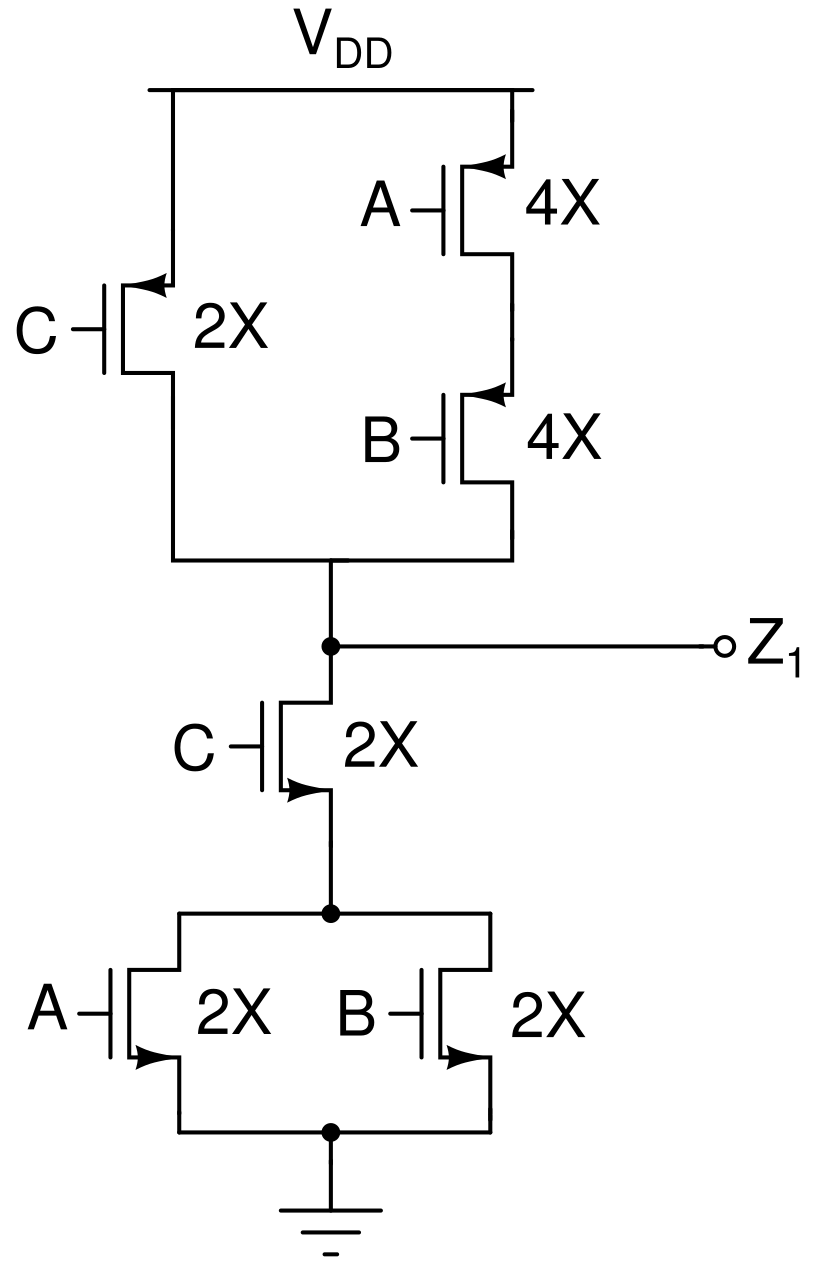
\includegraphics[width=0.5\textwidth]{figures/ece342_cc_q8_a.png}
        \end{figure}
        \newpage
    \item $Z_2 = \overline{(A \cdot B \cdot C) + (D \cdot E)}$ \\
    
    \textbf{Solution:}
        \begin{figure}[!h]
        \centering
        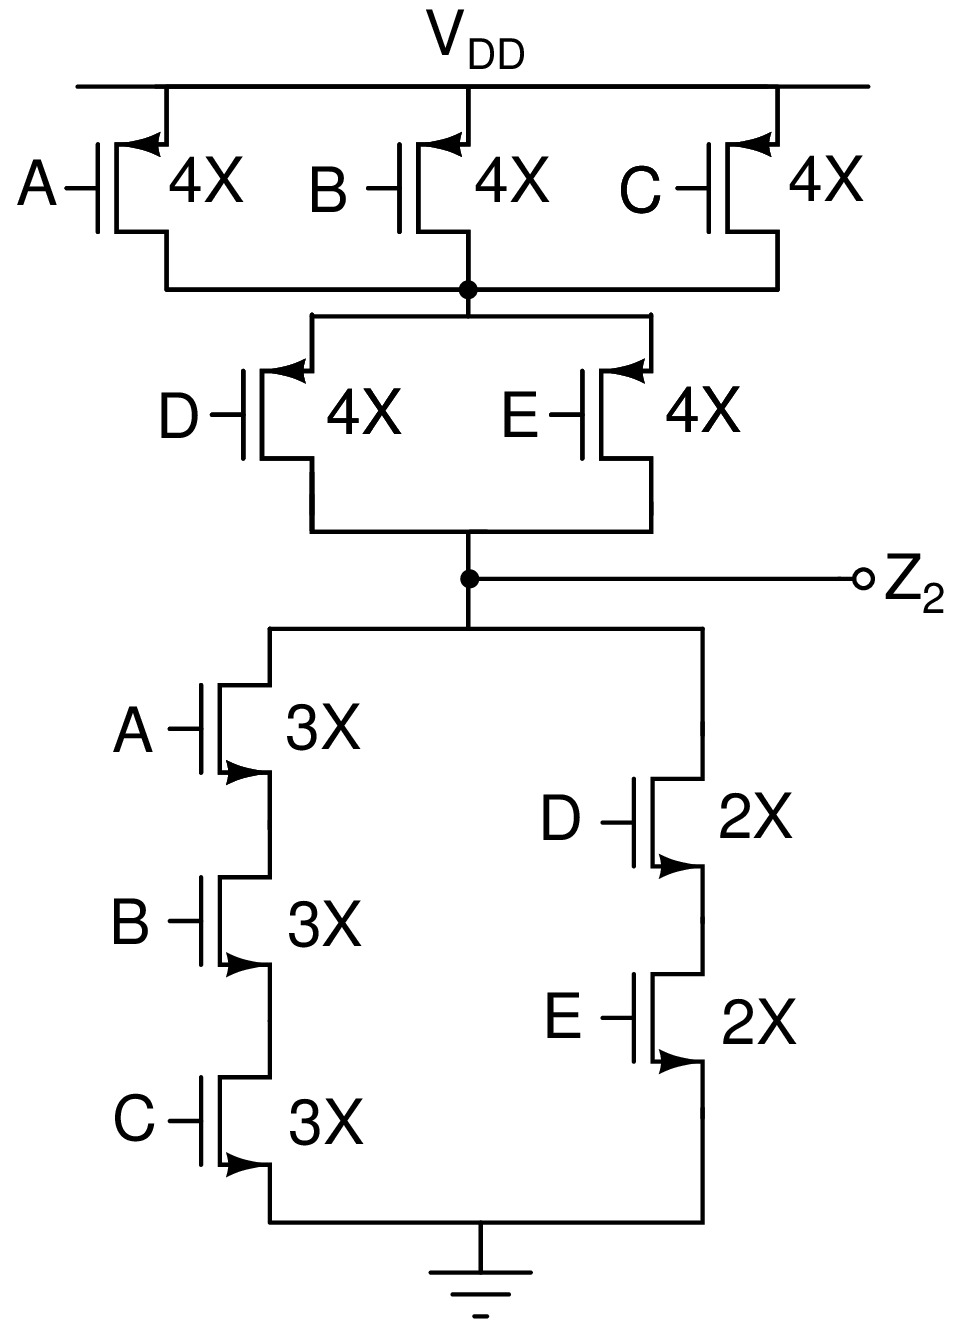
\includegraphics[width=0.5\textwidth]{figures/ece342_cc_q8_b.jpg}
        \end{figure}
\newpage
    \item $Z_3 = \overline{A} \cdot (\overline{B} + \overline{C} + \overline{D})$ \\
    
    \textbf{Solution:}
    $$\overline{Z_3} = \overline{\overline{A} \cdot (\overline{B} + \overline{C} + \overline{D})}$$
    $$\overline{Z_3} = A + \overline{(\overline{B} + \overline{C} + \overline{D})}$$
    $$\overline{Z_3} = A + (B \cdot C \cdot D)$$
    $$Z_3 = \overline{A + (B \cdot C \cdot D)}$$
    \begin{figure}[!h]
        \centering
        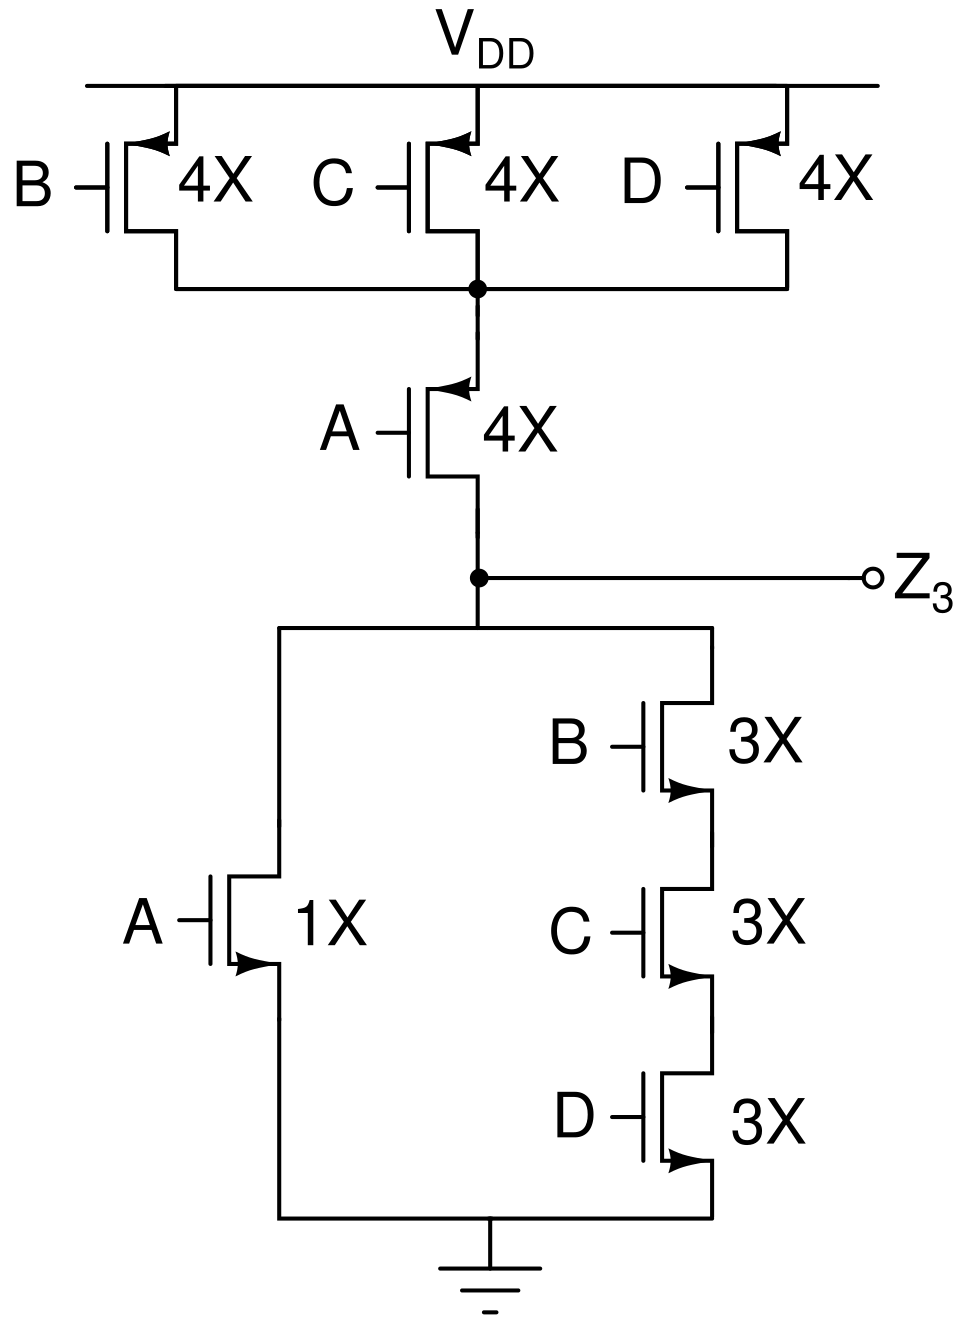
\includegraphics[width=0.5\textwidth]{figures/cc_cmos3.png}
        \end{figure}
\end{enumerate}

\end{document}